\documentclass{article}
\usepackage{xcolor}
\usepackage{graphicx}
\usepackage{microtype}
\usepackage{amsmath}
\usepackage{hanging}
% bottom must be 2in for printer
\usepackage[paperwidth=24in,paperheight=30in,top=1.5in,bottom=2in,left=1in,right=1.5in]{geometry}
\usepackage{fontspec}
\pagestyle{empty}
\begin{document}
\begin{minipage}[c]{20in}
{ 
\fontspec{DIN 1451 Std}[Color=gray, LetterSpace=4.0]
\fontsize{2.7in}{0.5in}\selectfont 
\bfseries

FAKE FONTS?
}\vspace{0.4in}\\
{ 
\fontspec{DIN 1451 Std}[Color=red, LetterSpace=2.0]
\fontsize{1.8in}{0.5in}\selectfont 
\bfseries
\vspace{0.5in}
EXPERIMENTS IN AI TYPE DESIGN

}
\end{minipage}
\vspace{0in}\\
\colorbox{white}{
\begin{minipage}{21.5in}
%\centering
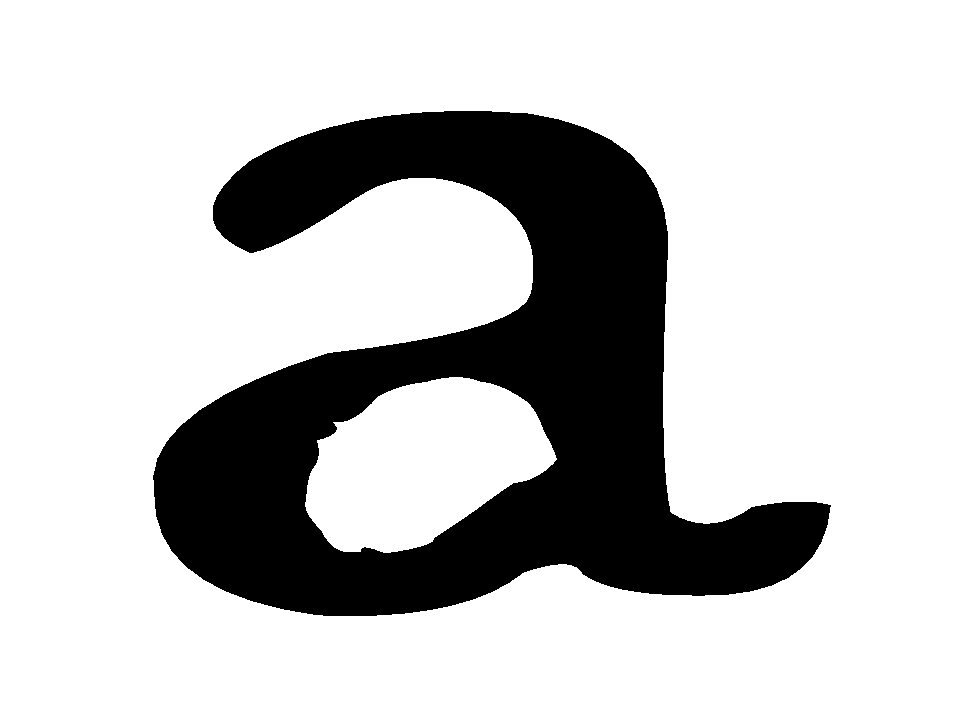
\includegraphics[width=6.5in,trim=40 0 40 0,clip]{a.pdf}
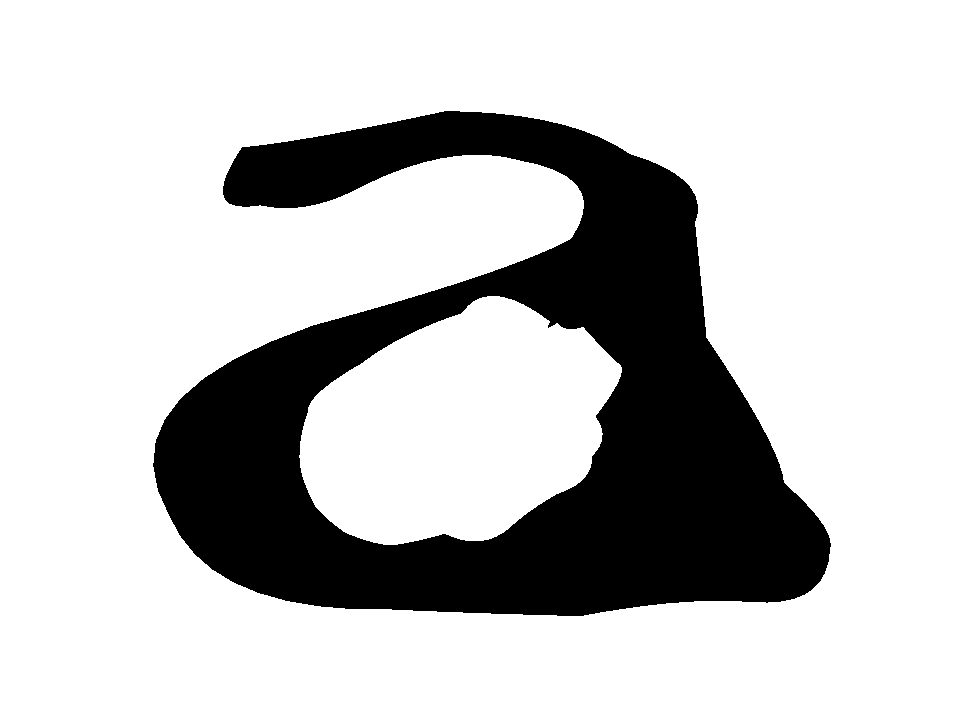
\includegraphics[width=6.5in,trim=40 0 40 0,clip]{a2.pdf}
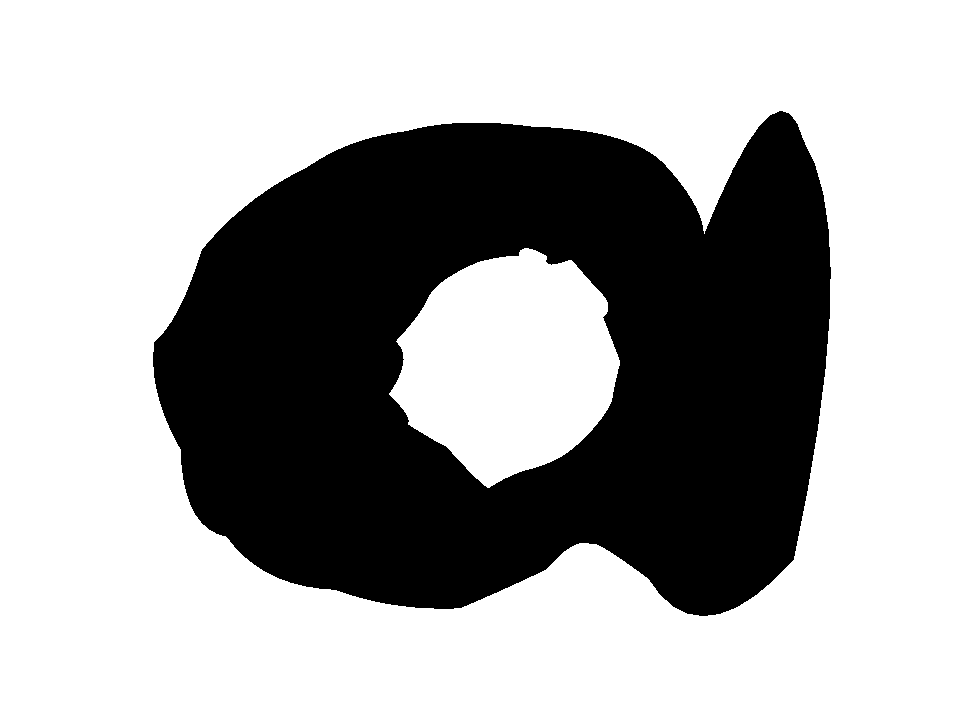
\includegraphics[width=6.5in,trim=40 0 40 0,clip]{a3.pdf}\vspace{-1in}\\
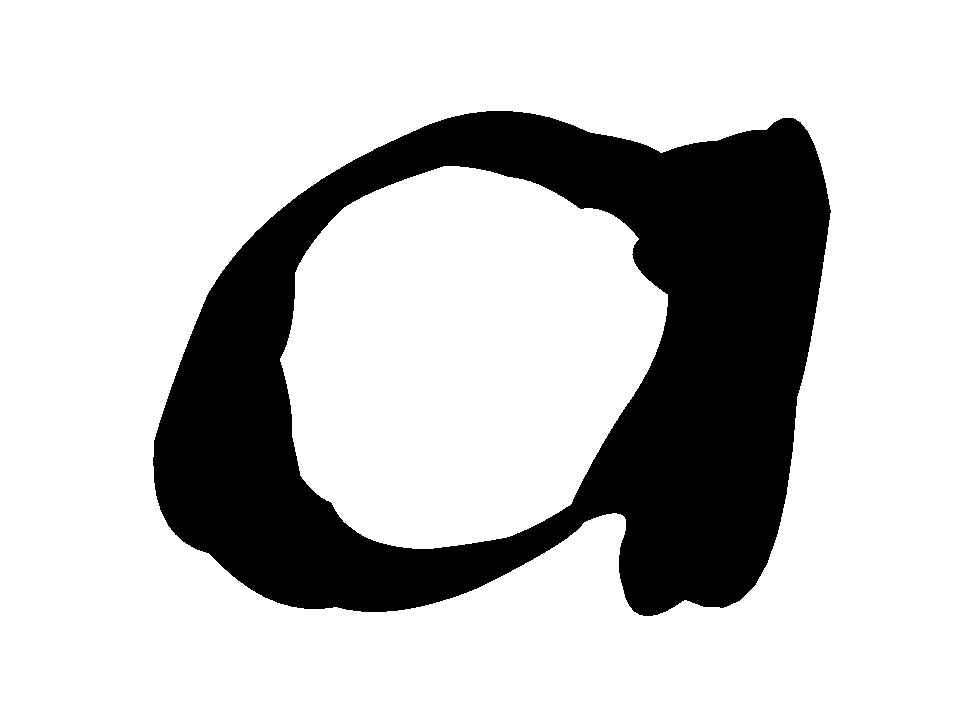
\includegraphics[width=6.5in,trim=40 0 40 0,clip]{a4.pdf}
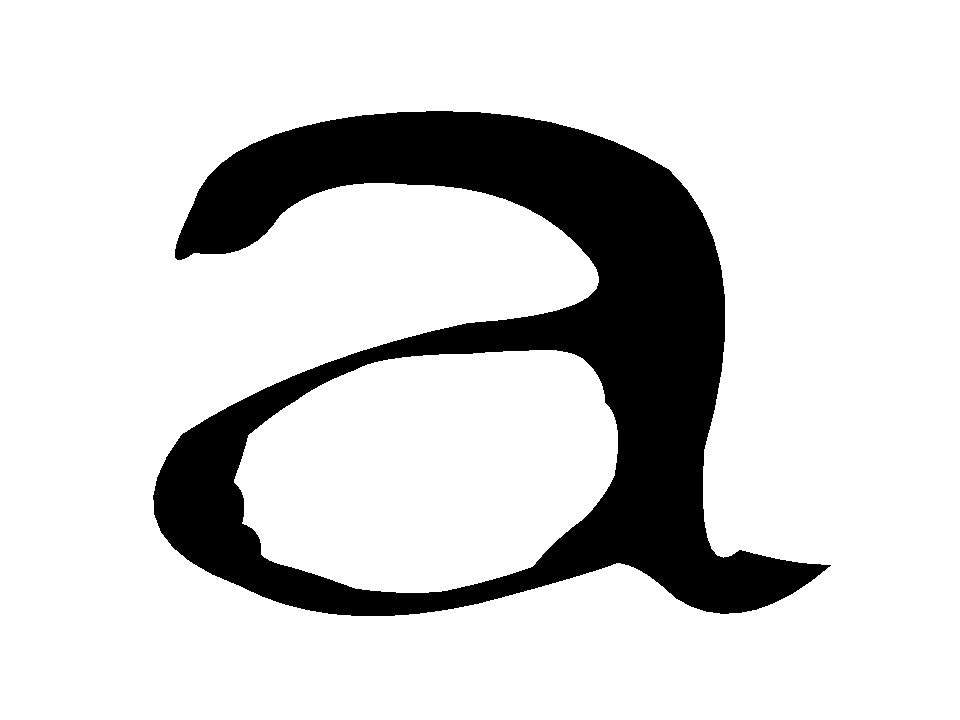
\includegraphics[width=6.5in,trim=40 0 40 0,clip]{a5.pdf}
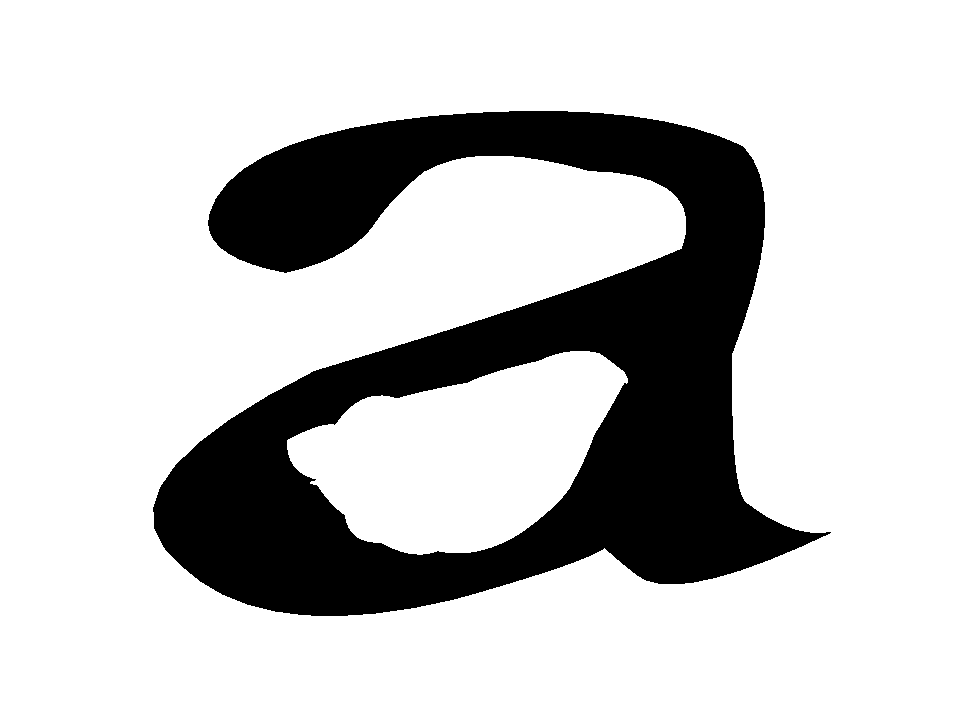
\includegraphics[width=6.5in,trim=40 0 40 0,clip]{a6.pdf}
\end{minipage}
}
\vspace{0.5in}\\
{
\fontspec{DIN 1451 Std}[Color=black]
\fontsize{1in}{1em}\selectfont 
ARIANA FREITAG
}
{
\fontspec{DIN 1451 Std}[Color=black]
\fontsize{0.8in}{1em}\selectfont 
EE '20,
}
{
\fontspec{DIN 1451 Std}[Color=black]
\fontsize{1in}{1em}\selectfont 
JONATHAN PEDOEEM
}
{
\fontspec{DIN 1451 Std}[Color=black]
\fontsize{0.8in}{1em}\selectfont 
EE '20,
}\vspace{0.2in}\\
{
\fontspec{DIN 1451 Std}[Color=black]
\fontsize{1in}{1em}\selectfont 
GEORGE HO
}
{
\fontspec{DIN 1451 Std}[Color=black]
\fontsize{0.8in}{1em}\selectfont 
BSE '19,
} 
{
\fontspec{DIN 1451 Std}[Color=black]
\fontsize{1in}{1em}\selectfont 
OSTAP VOYNAROVSKIY
}
{
\fontspec{DIN 1451 Std}[Color=black]
\fontsize{0.8in}{1em}\selectfont 
EE '19
}


\vspace{0.2in}

{
\fontspec{DIN 1451 Std}[Color=black]
\fontsize{0.8in}{1em}\selectfont 
\noindent ADVISOR: CHRIS CURRO
}

\vspace{0.5in}
\hspace*{.1in}
\begin{minipage}{10in}
  \sffamily
  \fontsize{0.63in}{0.74in}\selectfont \raggedright

  We are developing a neural network algorithm capable of generating
  new vector typefaces. By providing pre-existing typefaces made and
  designed by graphic designers to our models, they are capable of
  determining what letters ought to look like and how letters are
  structured into fonts --- through this process it generates Bézier
  curves which describe entirely new vector fonts.

\end{minipage}
\hfill
\begin{minipage}{10in}
  \sffamily
  \fontsize{0.6in}{0.7in}\selectfont
  \raggedright
  \vspace{-0.2in}
  The benefit of a vector based character is that a designer can place
  it directly in their work or manipulate it to their needs.
  \vspace{0.4in}

  We employ an autoencoder model and a generative adversarial
  network, aiming to consistently generate usable typefaces. The process
  can result in odd and unexpected shapes, some {\itshape a}'s
  we've generated have not looked like {\itshape a}'s at all!

  \vspace{0.4in}
  
  \fontsize{0.42in}{0.55in}\selectfont

  Source Code: {\ttfamily github.com/ccurro/font-bakers}\\
  Special Thanks: Cara Di Edwardo
\end{minipage}
\end{document}
